\chapter{Mathematical Preliminaries}

\section{Introduction to Numerical Methods}

Numerical methods are systematic procedures for obtaining approximate solutions to mathematical problems using a computer or calculator. They are especially useful when an exact analytic solution does not exist, is difficult to obtain, or is too complicated to be useful in practice.

A numerical computation usually contains the following:
\begin{enumerate}[leftmargin=1.5cm]
  \item a mathematical model or equation;
  \item an algorithm consisting of a finite sequence of steps;
  \item an approximation produced by the algorithm; and
  \item an assessment of the error and accuracy of that approximation.
\end{enumerate}

Unlike symbolic mathematics, numerical mathematics must also account for the fact that computers store only finitely many digits. Therefore, even an algebraically correct formula may give a poor numerical answer if it is evaluated carelessly.

\section{Types of Errors}

\begin{definition}[Basic errors]
Let $x$ be the true value and let $\widehat{x}$ be an approximation to $x$.
\begin{enumerate}[label=(\alph*),leftmargin=2.7em]
  \item The \emph{error} is
     $\quad e=x-\widehat{x}.$
  \item The \emph{absolute error} is
     $\quad |e|=|x-\widehat{x}|.$
  \item The \emph{relative error} is
     $\quad \varepsilon_r=\frac{x-\widehat{x}}{x},\qquad x\ne0.$
  \item The \emph{percentage relative error} is
  $\quad 100\varepsilon_r\% = \frac{x-\widehat{x}}{x} \times 100\%.$
\end{enumerate}
When only the magnitude matters, we consider the absolute relative error
\(\displaystyle{\frac{|x-\widehat{x}|}{|x|}.}\)
\end{definition}

\begin{definition}[Round-off error]
A \emph{round-off error} occurs because a computer or calculator represents a real number using only finitely many digits. Arithmetic performed with these finite representations may differ from exact real-number arithmetic.
\end{definition}

\begin{definition}[Truncation error]
A \emph{truncation error} results from replacing an exact mathematical process by a finite approximation. Examples include terminating an infinite series and replacing a derivative by a finite-difference formula.
\end{definition}

\newpage

\begin{example}[(Round-off error)]
Let
\[
  f(x)=\frac{x^2-\frac19}{x-\frac13}.
\]
Using four-digit arithmetic, evaluate $f(0.3334)$ directly and then by first algebraically simplifying the formula.
\end{example}

\begin{solution}[5.6cm]
Direct substitution in four-digit arithmetic gives
\[
  x^2\approx0.1112,\qquad \frac19\approx0.1111,
  \qquad x-\frac13\approx0.3334-0.3333=0.0001.
\]
Hence
\[
  f(0.3334)\approx\frac{0.1112-0.1111}{0.3334-0.3333}
  =\frac{0.0001}{0.0001}=1.
\]
Algebraically however,
\[
    f(x) = \frac{x^2-\frac19}{x-\frac13} = \frac{\left(x-\frac13\right)\left(x+\frac13\right)}{x-\frac13} = x + \frac13, \quad\text{for } x \neq \frac13
\]
Therefore
\[
  f(0.3334)=0.3334+0.3333=0.6667.
\]
and the round off error is
\[
    1 - 0.6667 = 0.3333.
\]
The direct formula subtracts nearly equal numbers in both numerator and denominator. This is an example of \emph{catastrophic cancellation}: small rounding errors are magnified by subtraction.
\end{solution}

\begin{example}[(Truncation error)]
Recall the Taylor series for $e^x$:
\[
 e^x=1+x+\frac{x^2}{2!}+\frac{x^3}{3!}+\cdots.
\]
If 
\(1+1+\frac1{2!}+\frac1{3!}+\cdots+\frac{1}{10!}\)
is used to approximate $e$, identify the truncation error.
\end{example}

\begin{solution}[2.8cm]
Since
\(
 e=1+1+\frac1{2!}+\frac1{3!}+\cdots,
\)
the omitted tail is
\[
 R=\frac1{11!}+\frac1{12!}+\frac1{13!}+\cdots.
\]
This infinite tail is the truncation error of the finite approximation.
\end{solution}

\newpage

\section{Taylor Series and Approximation}

\begin{theorem}[Taylor's Theorem]
Suppose that $f\in C^n[a,b]$ and that $f^{(n+1)}$ exists on $[a,b]$. Let $x_0\in[a,b]$. For every $x\in[a,b]$, there exists a number $\xi \in (x_0, x)$ such that
\[
  f(x)=P_n(x)+R_n(x), \quad
  P_n(x)=\sum_{k=0}^{n}\frac{f^{(k)}(x_0)}{k!}(x-x_0)^k, \quad
  R_n(x)=\frac{f^{(n+1)}(\xi)}{(n+1)!}(x-x_0)^{n+1}.
\]
where $P_n(x)$ is the $n$th-order Taylor polynomial, and $R_n(x)$ is the Lagrange remainder.
\end{theorem}

\bigskip

The Taylor polynomial $P_n(x)$ is used as an approximation to $f(x)$, while $R_n(x)$ is the associated truncation error. In applications, we want to find the upper bound for the magnitude of the truncation error (as we have learned in Calculus II):
\[
  |R_n(x)|\le
  \frac{M}{(n+1)!}|x-x_0|^{n+1},
\]
where $M$ can be considered as the absolute maximum of $f^{(n+1)}(x)$ on $(x_0, x)$.
\[
    \text{i.e.} \quad |f^{(n+1)}(t)|\le M \quad \text{for every } t \in (x_0, x)
\]

\begin{example}
Let $f(x)=\ln(1+x)$. Find the third-order Taylor polynomial $P_3(x)$ about $x_0=0$ and use it to estimate $\ln(1.2)$.
\end{example}

\begin{solution}[5.0cm]
\[
 f(x)=\ln(1+x), \qquad
 f'(x)=\frac1{1+x},\qquad
 f''(x)=-\frac1{(1+x)^2},\qquad
 f'''(x)=\frac2{(1+x)^3}.
\]
At $x_0=0$,
\[
 f(0)=0,\qquad f'(0)=1,\qquad f''(0)=-1,
 \qquad f'''(0)=2.
\]
Thus
\[
    P_3(x)=\sum_{k=0}^{3}{\frac{f^{(k)}(x_0)}{k!}(x-x_0)^k}=0+\frac{1}{1!}x-\frac{1}{2!}x^2+\frac{2}{3!}x^3=x-\frac{x^2}{2}+\frac{x^3}{3}.
\]
Then,
\(
 \ln(1.2) = \ln(1 + 0.2) \approx P_3(0.2)
 =0.2-\frac{0.2^2}{2}+\frac{0.2^3}{3}
 =0.182666\ldots\approx0.1827.
\)
\end{solution}

\medskip

\begin{example}
Estimate an upper bound for the truncation error when $P_3(0.2)$ is used to approximate $\ln(1.2)$.
\end{example}

\begin{solution}[4.2cm]
For $f(x)=\ln(1+x)$,
\[
    f^{(4)}(x)=\frac{d}{dx}f'''(x)=\frac{d}{dx}\frac{2}{(1+x)^3}=-\frac{6}{(1+x)^4}.
\]
On the interval $0\le x\le0.2$,
\[
 0 \leq x\leq 0.2 \implies 1 \leq (1+x)^4 \leq 1.2^4 \implies 
 \frac{1}{1.2^4} \leq \frac{1}{(1+x)^4} \leq 1.
\]
\(\displaystyle{ \therefore |f^{(4)}(x)|=\frac6{(1+x)^4}\le6.}\)

\medskip \noindent
\[
 \implies |R_3(0.2)| = \left|\frac{f^{(4)}(x)}{4!}(x-0)^4\right|
 \le\frac{6}{4!}|0.2|^4
 =\frac{6}{24}(0.0016)=0.0004.
\]
Hence, the upper bound for the truncation error in this case is $0.0004$.
\end{solution}

\section{Number Systems}

Humans normally use the decimal (or more technically, the base-$10$) number system. Computers store information using bits, or binary digits, so machine arithmetic is based on the binary, or base-$2$, system. Binary digits are often grouped in blocks of four and written in hexadecimal, or base-$16$, notation.

A very formal definition for a number in a base-$b$ number system is as follows:

\noindent
For a positional number system with base $b$,
\[
 (a_na_{n-1}\cdots a_0.a_{-1}a_{-2}\cdots)_b
 =\sum_{k=-\infty}^{n}a_kb^k,
\]
where each digit satisfies $0\le a_k<b$.

\bigskip
The following is a conversion table for decimal, binary, and hexadecimal numbers:

\begin{center}
\renewcommand{\arraystretch}{1.15}
\begin{tabular}{c*{8}{>{\centering\arraybackslash}p{1.05cm}}}
\toprule
Decimal & 0&1&2&3&4&5&6&7\\
Binary & 0000&0001&0010&0011&0100&0101&0110&0111\\
Hexadecimal & 0&1&2&3&4&5&6&7\\
\midrule
Decimal & 8&9&10&11&12&13&14&15\\
Binary & 1000&1001&1010&1011&1100&1101&1110&1111\\
Hexadecimal & 8&9&A&B&C&D&E&F\\
\bottomrule
\end{tabular}
\end{center}

To convert any decimal integer to a number of any other bases, we perform repeated division and keep track of the remainders as we do so. Then, the converted number is read from bottom to top (Example 5(a)).

\medskip
Converting to base-10 can be done by summing up the digits multiplied by the base raised to the power of its position number (Example 5(b),(d)).

\medskip
There also is a trick to convert a base-2 number to other bases of powers of 2. You perhaps have seen this trick in secondary school (if you took ASK) when converting binary, octal (base-8), and hexadecimal numbers. 
To convert from binary (base-2) to base-$2^k$, we group $k$ digits together and perform the corresponding conversions to each of the groups of digits (Example 5(c)). In this course, we will only handle decimal, binary, and hexadecimal numbers however.

\begin{example}
Perform the following conversions.
\begin{enumerate}[label=(\alph*),leftmargin=2.6em]
  \item Convert $1234_{10}$ to binary.
  \item Convert $10011010010_2$ to decimal.
  \item Convert $10011010010_2$ to hexadecimal.
  \item Convert $4D2_{16}$ to decimal.
\end{enumerate}
\end{example}

\newpage
\begin{solution}[8.0cm]
\begin{enumerate}[label=(\alph*),leftmargin=2.6em]
\item
\[
\begin{array}{r|r|c}
\div & \text{quotient} & \text{remainder}\\
\hline
2 & 1234 & 0\\
2 &  617 & 1\\
2 &  308 & 0\\
2 &  154 & 0\\
2 &   77 & 1\\
2 &   38 & 0\\
2 &   19 & 1\\
2 &    9 & 1\\
2 &    4 & 0\\
2 &    2 & 0\\
2 &    1 & 1\\
\cline{1-2}
2 &    0 & \\
\end{array}
\]
$\therefore 1234_{10}=10011010010_2.$
\item $10011010010_2=2^{10}+2^7+2^6+2^4+2^1=1234_{10}.$
\item Grouping the bits from the right in blocks of four,
\[
 10011010010_2=0100\;1101\;0010_2=4D2_{16}.
\]
\item $4D2_{16}=4(16^2)+13(16)+2=1024+208+2=1234_{10}.$
\end{enumerate}
\end{solution}

For numbers in bases other than 10 that have a point (e.g. $1.01_{2}$, $A.42_{16}$), we call them fractional base-$k$ numbers.

To convert them to base-10, we separate the digits into 2 groups, the digits before the point and digits after the point. For digits before the point, we repeatedly divide until we get 0 as we have discussed previously. For digits after the point, we repeatedly \emph{multiply} the fractional (or decimal) part while recording the whole number part. Similarly, we stop when the fractional part reaches 0.

As for converting fractional numbers \textit{to} base-10, we sum up the powers of the base according to its position number like before; just that now numbers after the point have a \textit{negative} power.

The trick for base-$2^k$ fractional numbers still work too, we just need to group numbers around the point.

\begin{example}
Convert $11011.0110_2$ to decimal and hexadecimal.
\end{example}

\begin{solution}[4.0cm]
For the decimal conversion,
\[
\begin{aligned}
11011.0110_2
 &=2^4+2^3+2^1+2^0+2^{-2}+2^{-3}\\
 &=16+8+2+1+\frac14+\frac18\\
 &=27.375_{10}.
\end{aligned}
\]
For the hexadecimal conversion, group into blocks of four around the binary point:
\[
 11011.0110_2=0001\;1011.0110_2=1B.6_{16}.
\]
\end{solution}

We should also consider infinite decimals (repeating and non-repeating) when discussing the conversion algorithm between different number bases.
Thus, we will use the idea of significant figures and rounding as we did in base-10.
In base-$k$, we round up if the following digit is $\geq k/2$ and vice versa.

\medskip
\noindent Note: In this course, we start counting significant digits immediately after the point.

\begin{example}
    Convert $\displaystyle{\frac13}$ to a binary number of three significant figures. Find the absolute round-off error.
\end{example}

\begin{solution}[4.1cm]
\[
\begin{array}{r|r|c}
\times & \text{fractional part} & \text{carry}\\
\hline
  & 1/3 & \\
2 & 2/3 & 0\\
2 & 1/3 & 1\\
2 & 2/3 & 0\\
2 & 1/3 & 1\\
\vdots & \vdots & \vdots
\end{array}
\]

$\therefore \displaystyle{\frac13=0.0101\ldots_2.}$

\medskip
Since we want three significant figures, 
\[
 \frac13\approx0.011_2=\frac38=0.375_{10}.
\]
Thus the absolute round-off error is
\[
 \left|\frac13-\frac38\right|=\frac1{24}
 =0.041666\ldots\approx0.0417.
\]
\end{solution}

We also consider an alternative method in solving the above example.

\begin{solution}[4.0cm]
We begin by multiplying $\displaystyle{\frac13}$ by $2^3$ since we want 3 significant figures.
Thus, we have:
\begin{align*}
    \frac13 \times 2^3 = \frac83 &= 2.67 \approx 3_{10} = 11_2 \\
    \implies \frac13 &= 11_2 \times 2^{-3} = 0.011_2
\end{align*}
And the absolute round-off error is $\displaystyle{\left|\frac13 - (3 \times 2^{-3})\right| \approx 0.0417}$.
\end{solution}

Notice that in the alternative method discussed above, we are able to work with a round number instead of needing to repeatedly multiply fractional parts.

\section{IEEE Floating-Point Numbers}

A computer has only finite memory, so it stores a real number using a finite floating-point representation. Common formats are:
\begin{itemize}
  \item $32$ bits: \emph{single precision};
  \item $64$ bits: \emph{double precision}.
\end{itemize}

A commonly used floating-point standard is the \textbf{IEEE 754} standard:
\[
  r=(-1)^s \times 2^q \times m,
\]
where $s$ is the sign bit, $q$ is the true exponent, and $m$ is the mantissa.

\noindent
The true exponent is $q = e - b$, where $e$ is the exponent and $b$ is the bias.

\subsection{IEEE 754 Single Precision}

A normalized single-precision number uses 32-bit memory; one sign bit, eight exponent bits, and twenty-three fraction bits:

\begin{center}
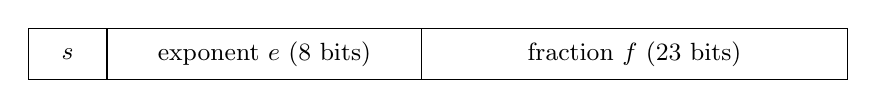
\begin{tikzpicture}[x=1cm,y=1cm]
  \draw (0,0) rectangle (1.00,0.65);
  \draw (1.00,0) rectangle (5.00,0.65);
  \draw (5.00,0) rectangle (10.4,0.65);
  \node[font=\small] at (0.50,0.325) {$s$};
  \node[font=\small] at (3.00,0.325) {exponent $e$ (8 bits)};
  \node[font=\small] at (7.70,0.325) {fraction $f$ (23 bits)};
\end{tikzpicture}
\end{center}


\noindent
For a normalized value,
\[
  fl(r)=(-1)^s2^{e-127}(1.f)_2.
\]
The bias, $b$ is $127$.

\begin{example}
Write $x=-1234$ in IEEE 754 single-precision floating-point representation and hexadecimal form.
\end{example}

\begin{solution}[6.5cm]
Converting $1234_{10}$ to binary:
\[
 1234_{10}=10011010010_2
 =1.0011010010_2\times2^{10}.
\]
Therefore
\[
 s=1,
 \qquad e=10+127=137=10001001_2.
\]
The fraction field is the part after the leading $1$:
\[
 f=00110100100000000000000.
\]
Hence the $32$ bits are
\[
 \underbrace{1}_{s}\;
 \underbrace{10001001}_{e}\;
 \underbrace{00110100100000000000000}_{f},
 \text{ or }
 11000100100110100100000000000000_2.
\]
Grouping into blocks of four gives
\[
 1100\;0100\;1001\;1010\;0100\;0000\;0000\;0000
 =\boxed{\texttt{C49A4000}}.
\]
\end{solution}

\begin{example}
Given $x=4.375_{10}=100.011_2$, convert $x$ to IEEE 754 single precision and give the answer in hexadecimal form.
\end{example}

\begin{solution}[5.5cm]
In scientific notation, we have:
\[
 100.011_2=1.00011_2\times2^2.
\]
Thus
\[
 s=0,
 \quad e=2+127=129=10000001_2,
\quad f=00011000000000000000000.
\]
The bit pattern is
\[
 0\;10000001\;00011000000000000000000.
\]
Grouping into hexadecimal digits,
\[
 0100\;0000\;1000\;1100\;0000\;0000\;0000\;0000
 =\boxed{\texttt{408C0000}}.
\]
\end{solution}

\subsection{IEEE 754 Double Precision}

A normalized double-precision number uses one sign bit, eleven exponent bits, and fifty-two fraction bits:

\begin{center}
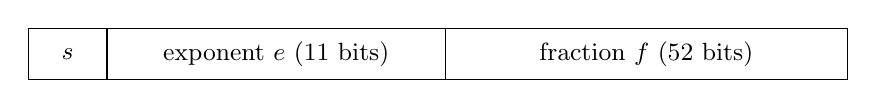
\begin{tikzpicture}[x=1cm,y=1cm]
  \draw (0,0) rectangle (1.00,0.65);
  \draw (1.00,0) rectangle (5.30,0.65);
  \draw (5.30,0) rectangle (10.4,0.65);
  \node[font=\small] at (0.50,0.325) {$s$};
  \node[font=\small] at (3.15,0.325) {exponent $e$ (11 bits)};
  \node[font=\small] at (7.85,0.325) {fraction $f$ (52 bits)};
\end{tikzpicture}
\end{center}

For a normalized value,
\[
  fl(r)=(-1)^s2^{e-1023}(1.f)_2.
\]
The bias, $b$ is $1023$.

\begin{example}
Convert the following IEEE 754 double-precision machine number to decimal:
\[
0100000000111011100100010000000000000000000000000000000000000000
\]
\end{example}

\begin{solution}[5.8cm]
Separate the fields:
\[
 s=0,
 \qquad e=10000000011_2=1027,
\]
and the fraction begins
\[
 f=1011100100010000\ldots.
\]
The true exponent is
\[
 q=e-1023=1027-1023=4.
\]
The significand is
\[
\begin{aligned}
(1.f)_2
 &=1.101110010001_2\\
 &=1+2^{-1}+2^{-3}+2^{-4}+2^{-5}+2^{-8}+2^{-12}\\
 &=1.722900390625.
\end{aligned}
\]
Therefore
\[
 r=2^4(1.722900390625)=\boxed{27.56640625}.
\]
\end{solution}

\begin{remark}
IEEE 754 also reserves exponent patterns for zero, subnormal numbers, infinities and NaN (Not a Number). The formulas above apply to normalized finite numbers.
\end{remark}

\section{Algorithms, Convergence and Accuracy}

An algorithm is a procedure that describes a finite sequence of steps performed in a specified order to solve a problem or produce a good approximation of the solution of said problem.

Many numerical algorithms are iterative. Starting from an initial approximation $x_0$, they generate a sequence
\[
    \{x_n\} = \{x_0,x_1,x_2,\ldots\}
\]
by repeatedly applying an update formula $f(x) \text{ s.t. } x_{i+1} = f(x_i)$. Main concepts are:
\begin{itemize}
  \item \textbf{initial condition}: the starting approximation or initial guess $x_0$;
  \item \textbf{iteration}: applying the algorithm $x_{i+1} = f(x_i)$;
  \item \textbf{convergence}: for a sufficiently large $N$, $x_N$ approach a limiting value;
  \item \textbf{stopping criterion}: a rule for deciding when the approximation is sufficiently accurate.
\end{itemize}

\noindent
Common stopping criteria include
\[
 |x_n-x_{n-1}|<\epsilon,
 \qquad
 \left|\frac{x_n-x_{n-1}}{x_n}\right|<\epsilon,
 \qquad
 |f(x_n)|<\epsilon,
\]
where $\epsilon$ denotes a sufficiently small error.
Sometimes, we also include a maximum allowed number of iterations.

\begin{example}
Find an approximate root of
\[
 x^2-5x+6=0.
\]
\end{example}

\begin{solution}[9.0cm]
An algorithm to estimate the root of $x^2 -5x +6 =0$ is the Newton-Raphson Method (to be covered in Chapter 3).

\noindent
We first choose an initial guess $x_0$. Let $x_0 = 0$.

\noindent
Then let
\[
 f(x)=x^2-5x+6,
 \qquad f'(x)=2x-5.
\]
Then, we improve the guess by Newton's formula:
\[
 x_{n+1}=x_n-\frac{f(x_n)}{f'(x_n)}
 =x_n-\frac{x_n^2-5x_n+6}{2x_n-5}.
\]
Repeatedly applying the formula until desirable accuracy, we have:
\[
\begin{array}{c|c}
\toprule
n & x_n\\
\midrule
0&1.000000\\
1&1.666667\\
2&1.933333\\
3&1.996078\\
4&1.999985\\
5&2.000000\\
\bottomrule
\end{array}
\]
Thus, the sequence converges to the root $x=2$.

\bigskip \noindent
Checking the exact solution, our above equation factors as:
\[
 x^2-5x+6=(x-2)(x-3),
\]
so the exact roots are $2$ and $3$.

\bigskip \noindent
Looking at our approximation and accuracy at $n=4$, the absolute error relative to the exact root is approximately
\[
 |2-x_4| = |2-1.999985|\approx1.5\times10^{-5}.
\]
A practical implementation would stop once a prescribed stopping criteria (e.g. a tolerance or error, $\epsilon$, or usually an approximation of such an error) is met, or once a given maximum iteration count is reached.
\end{solution}

\begin{remark}
Convergence is not guaranteed merely because an iterative formula can be written down. The choice of algorithm, initial approximation and stopping criterion can all affect whether the computed sequence converges and how quickly it does so.
\end{remark}

\bigskip

In the upcoming chapters, we will explore a handful of algorithms to approximate a solution to a few different types of problems.

\phantomsection
\section*{Tutorial 1}
\addcontentsline{toc}{section}{Tutorial 1}

\begin{enumerate}[
    label=\arabic*.,
    leftmargin=1.5em,
    itemsep=0.4em,
    parsep=0.1em
]

    \item Let \(f(x)=\sqrt{x+1}\).
    \begin{enumerate}[
        label=(\alph*),
        leftmargin=2em,
        itemsep=0pt,
        topsep=0.2em,
        parsep=0pt,
        partopsep=0pt
    ]
        \item Find the third-order Taylor polynomial \(P_3(x)\)
        about \(x_0=0\).
        \item Use \(P_3(x)\) to approximate
        \(\sqrt{0.5}\) and \(\sqrt{1.25}\).
        \item Find the absolute errors of the approximations in part~(b).
    \end{enumerate}

    \item Let \(f(x)=\cos x\).
    \begin{enumerate}[
        label=(\alph*),
        leftmargin=2em,
        itemsep=0pt,
        topsep=0.2em,
        parsep=0pt,
        partopsep=0pt
    ]
        \item Find the third-order Taylor polynomial \(P_3(x)\)
        for the function \(f(x)\) about \(x_0=0\).
        \item Find an upper bound for the truncation error when
        approximating \(\cos(0.01)\) using the polynomial obtained
        in part~(a).
    \end{enumerate}

    \item
    \begin{enumerate}[
        label=(\alph*),
        leftmargin=2em,
        itemsep=0pt,
        topsep=0pt,
        parsep=0pt,
        partopsep=0pt
    ]
        \item Convert the decimal number \(5432_{10}\) to a binary number.
        \item Convert the binary number
        \(1010100111000_2\) to a decimal number.
        \item Convert the binary number
        \(1010100111000_2\) to a hexadecimal number.
        \item Convert the hexadecimal number
        \(1538_{16}\) to a decimal number.
    \end{enumerate}

    \item Convert each of the following binary numbers into decimal
    and hexadecimal numbers.
    \begin{enumerate}[
        label=(\alph*),
        leftmargin=2em,
        itemsep=0pt,
        topsep=0.2em,
        parsep=0pt,
        partopsep=0pt
    ]
        \item \(110011.011010_2\)
        \item \(11100010.100111_2\)
    \end{enumerate}

    \item Convert \(\dfrac{1}{3}\) to a binary number of eight significant
    digits. Find the round-off error.

    \item Convert the decimal number \(12345_{10}\) to the IEEE~754
    single-precision floating-point format.

    \item Given that
    \[
        x=10001110011.00011_2,
    \]
    convert \(x\) to the IEEE~754 single-precision floating-point
    representation. Express the answer in hexadecimal form.

    \item Convert the machine number
    \[
        01000001101110010000000000000000
    \]
    to a decimal number.

\end{enumerate}
